%%% Ch. 5: Discussion & Analysis%%%
\chapter{Discussion \& Analysis} \label{ch:discussion}
%The endorsement system provides a method to assign a reputation score (\ac{TEI}) to each individual entities based on the endorsement interaction in the system. By specifying the interactions between entities via smart contracts code and deploying the contract code on blockchain network, a decentralized application for endorsement system was developed. 
%As a decentralied and distributed system  
%
%f


%This chapter discusses the fulfillment of the project goal. The answers to the
%research questions posed at the beginning of this project are answered
%theoretically as well as implementation wise as necessary.\\
%
%\textbf{Research question 1: }How can graph theories and relevant reputation
%algorithms be used to model the interaction between entities and
%detect/identify honest and malicious nodes in the network? How can the
%interaction graph be modeled? \\
%
%This is answered by section ~\ref{sec:interaction},
%~\ref{sec:threatModel}.\\
%
%\textbf{Research question 2: }What are the requirements for storing trust values
%and linking them to associated identities stored off a blockchain network? How
%can a blockchain application be built to define a general trust framework for a
%transactional network? How could the overall system architecture look like?\\
%
%This is answered by section ~\ref{sec:endorsementModel},
%~\ref{ch:UserStories}, ~\ref{subsec:design_considerations}
%~\ref{sec:pocDesign}. \\
%
%\textbf{Research question 3: }How can the discussed endorsement network ensure
%trustworthiness while also preserving users anonymity and how can it be
%generalized to other transactional network or added on top of it to serve other
%use cases such as content filtering, E-Commerce, etc.? \\
%
%This is answered by section ~\ref{subsec:bcConsensus},
%~\ref{sec:generalization}.\\
%
%%\section{Contract calls with web browser}
%%Additionally, frontend was deployed using Reactjs and web3 API to communicate
%%with smart contracts on blockchain directly from the browser. \\
%%The features implemented were: \\
%%\begin{itemize}
%%	\item View list of all participants: Anyone can see the list of all
%%	participants registered on endorsement network. This feature relates to
%%	requirement R3. Figure ~\ref{listall} demonstrates this feature.   
%%	\begin{figure}[h]
%%		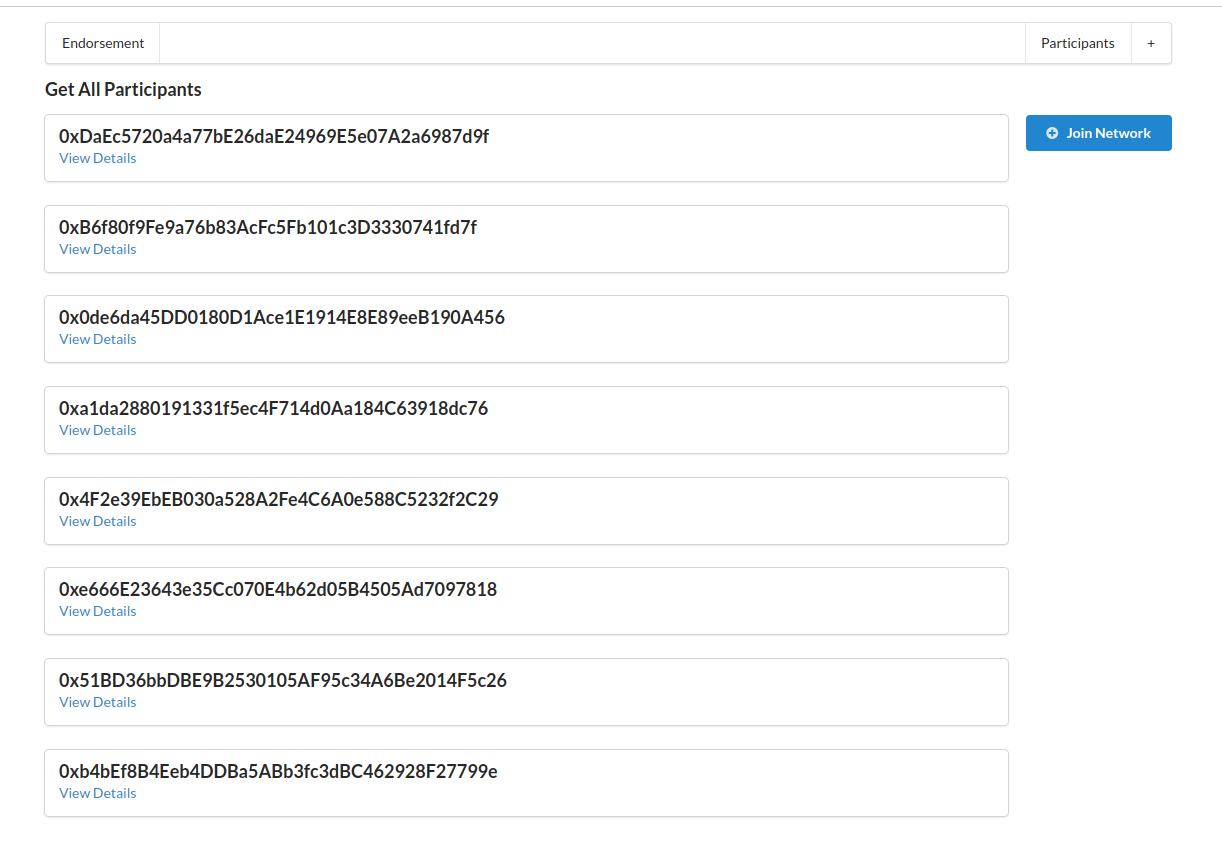
\includegraphics[width=0.95\textwidth]{Images/1_Frontend.eps} 
%%		\caption{List of all participants} 
%%		\label{listall}
%%	\end{figure}
%%	\item Join Network with a Pseudonym: Anyone can join the endorsement
%%	network and start calling the send/remove endorsement functions from the
%%	endorsement contract. This feature relates to requirement R4.2. Figure ~\ref{joinNetwork} demonstrates this feature. 
%%	\begin{figure}[h]
%%		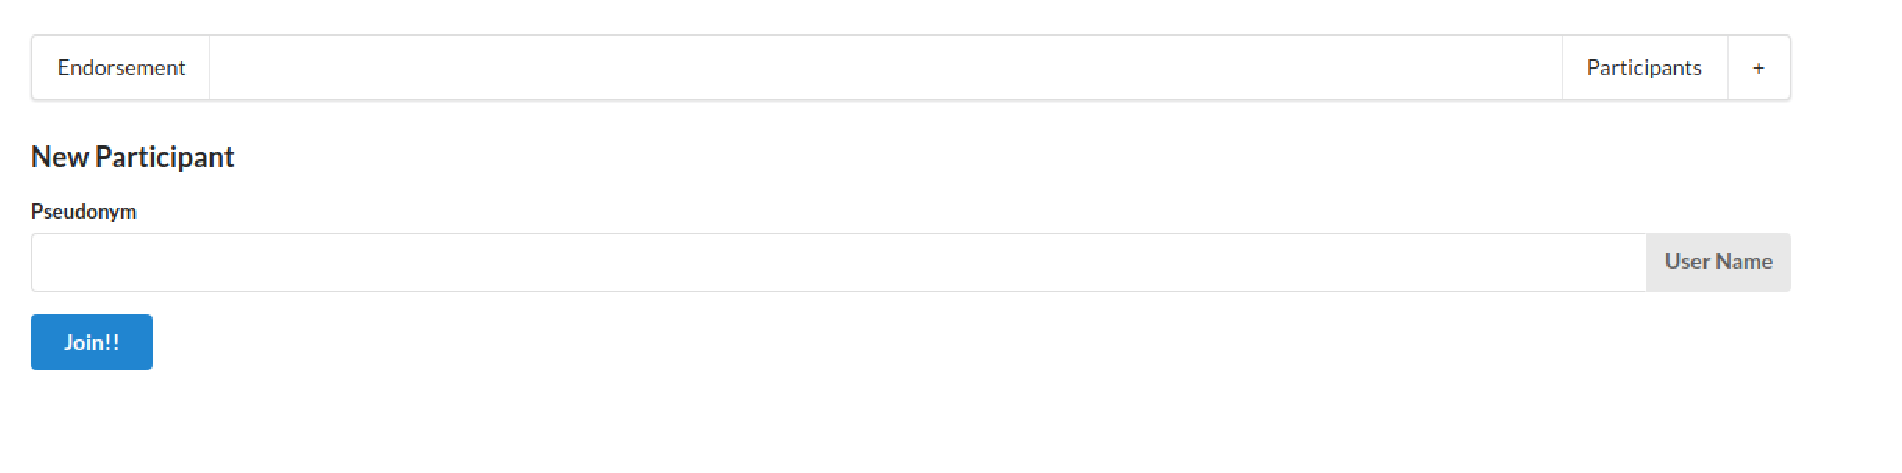
\includegraphics[width=0.95\textwidth]{Images/2_Frontend_JoinNetwork.eps} 
%%		\caption{Join Network using Pseudonym} 
%%		\label{joinNetwork}
%%	\end{figure}
%%	\item Send and Remove Endorsement: Anyone can view the details of all
%%		registered participants on the network which is a requirement mentioned
%%		by R3, R4. However, sending and removing endorsement checks if the
%%		message sender is a registered participant or not. Only if it's true,
%%		then the sending or removing of endorsement is called without error.
%%		This feature refers to requirement R1 and R2. Figure ~\ref{viewDetails}
%%		shows the view details of participants along with the send and remove
%%		endorsement feature.
%%		\begin{figure}[h]
%%			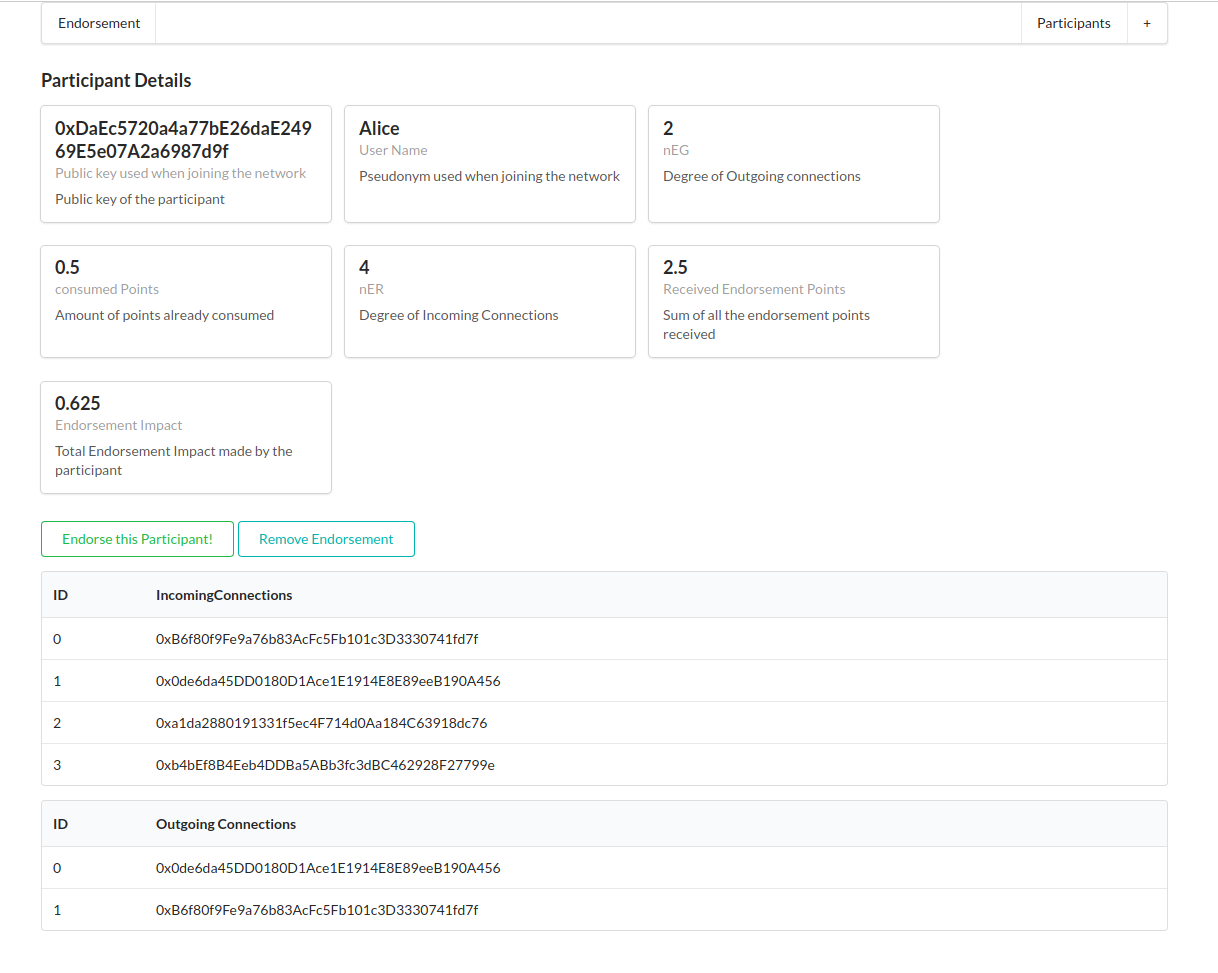
\includegraphics[width=0.95\textwidth]{Images/3_Frontend_ViewDetails.eps} 
%%			\caption{View Details of participants and endorse them} 
%%			\label{viewDetails}
%%	\end{figure}
%%\end{itemize}
%%
%%\section{Generalization} \label{sec:generalization}
%%The endorsement PoC is a general model that aggregates and assign reputation
%%scores to individuals based on their interaction in a network. As such, any
%%transactional network, e-commerce, content-serving platform, etc. can use it.
%%The platform-specific reputation system can still co-exist alongside the
%%endorsement model. It is useful to get an objective measure of the actual
%%transaction feedback(history, quality of services, etc.).  Consider a buy/sell
%%system scenario where two unknown entites, A and B are attempting to transact
%%with each other. The entities can check each other's rating/feedback from the
%%platform's reputation system in use. If that is not enough for deciding on the
%%transaction, they can check the endorsement network for the global reputation
%%score of the entity in question. As such, the decision is no more reliant only
%%on A's reputation or the platform's reputation. There is a third option that
%%guarantees a reliable and immutable data stored in a decentralized manner. From
%%the view of the platform, say, B/S, it allows users on endorsement network to
%%transact on B/S. The users of B/S gets output from decentralized trust score
%%storage system. The platform itself provides input to the endorsement system in
%%case of a failed transaction outcome to help penalize the peer in the
%%endorsement network. Doing so increases the accuracy in both systems. 
%%
%%
%%%The results presented in Chapter 4 are discussed and analyzed, including comments and reflections from the author. It may include the following: Comparison of obtained results with discussion,interpretation and evaluation of results. Results of analysis or modeling are described. Interpretations are drawn and connected to previous work
